\setcounter{chapter}{1}

\chapter{Background}\label{cha:background}
In this chapter, we briefly review web services, then we introduce
the concept of communities of web services, their architecture and
applications and the benefits of forming communities. Thereafter,
we discuss the cooperative game theory concepts used throughout
the thesis. Finally, we discuss relevant related work on web
service communities and games in the literature of service
oriented computing.

\section{Community of Web Services}\label{sec:CommunityWS}
In this section, we present web services and discuss the concept
of their communities from architectural and operations
perspectives.

\subsection{Web Services}\label{sec:CWSWebServices}
Over the past years, online services have become part of standard
daily life of people around the globe. Many modern applications
rely on web services from different providers. For instance, many
mobile and tablet applications which have limited storage and
processing power are merely interfaces aggregating different
information from online services. Examples are vast, weather
forecasting, ticket selling, shopping apps, local maps and places
searching are some of them.

The World Wide Web Consortium (W3C) defines web services as
follows: ``software system designed to support interpretable
machine-to-machine interaction over a network. It has an interface
described in a machine-processable format (specifically WSDL).
Other systems interact with the web service in a manner prescribed
by its description using SOAP messages, typically conveyed using
HTTP with XML serialization in conjunction with other Web-related
standards''. When developers declare a new web service, it will be
discovered based on its description that fully discloses its
functionalities. Developers also have to declare a public
interface and a readable documentation to help other developers
when integrating different services \cite{w3cwsdl}. Nowadays, web
API standards which do not require XML-based web service protocols
like SOAP and WSDL are also emerging. They are also called REST
(representational state transfer) services which are moving
towards simpler communication protocols. %They are not restricted
%to XML formats, recently JSON, a human readable and simpler format
%is becoming popular among online service providers.

We are not going to delve into engineering details of online web
service implementation and its protocols in this thesis. We are
interested in web services from their business model perspective.
Service providers usually charge end users for services they
provide. For example, Google has listed their pricing and plans
for wide range of services they provide on their web service
console page\footnote{https://code.google.com/apis/console}.

In our research work, we abstract web services as rational
agents\footnote{The term
        rational is used here in the sense that web services are utility
        maximizers} providing services to end users. They aim to maximize
        their individual income by receiving enough requests from end
        users. In order to increase their revenue, web services seek for
        more tasks if they have the capacity and throughput to do so. Web
        services can join communities to have better efficiency by
        collaborating with others, to have access to broad market share,
        and to have opportunity of receiving a bigger task pool from end
        users. Furthermore, the high reliance on web services has increased quality expectations from end users.
        Communities of web services can provide higher availability, performance, reliability, and recovery for end users.

\subsection{Web Services Communities}\label{sec:CWSDefinition}
Community refers to ``the condition of sharing or having certain
attitudes and interests in common'' or ``a group of people living
in the same place or having a particular characteristic in
common''\footnote{Oxford Dictionaries}. In
\cite{DBLP:journals/internet/BenatallahSD03,
Zeng:2003:QDW:775152.775211}, the authors introduce community of
web services as collection of cooperative web services with common
functionalitiers but different QoS metrics. Therefore
$communities$ are differentiated from $composition$ types of web
service cooperation in which web services with different
functionalities work together to generate a new service with
composite functionality.


Maamar et al. initially in \cite{conf/webist/MaamarLBTS07} and
then comprehensively in \cite{DBLP:journals/ijebr/MaamarSTBB09}
proposed an architecture utilizing \emph{Contract-Net} protocol
for engineering task distribution within communities. This
architecture has been further developed in
\cite{conf/IEEEscc/BenharrefSBB11, conf/IEEEscc/KhosravifarBMMT10,
conf/aina/LimTM11, CSTintercommunity}. Two types of roles have
been distinguished for community members: masters and slaves.
Master web services lead communities and are responsible for
membership management. They can invite and convince slave web
services to join the community, and attract new slave web services
to their communities by awarding them better payoff. Moreover,
they can eject some slave members from the community to improve
its overall reputation if these members are misbehaving or cannot
provide the promised QoS \cite{DBLP:journals/ijebr/MaamarSTBB09}.

        \begin{figure}
            \begin{center}
%            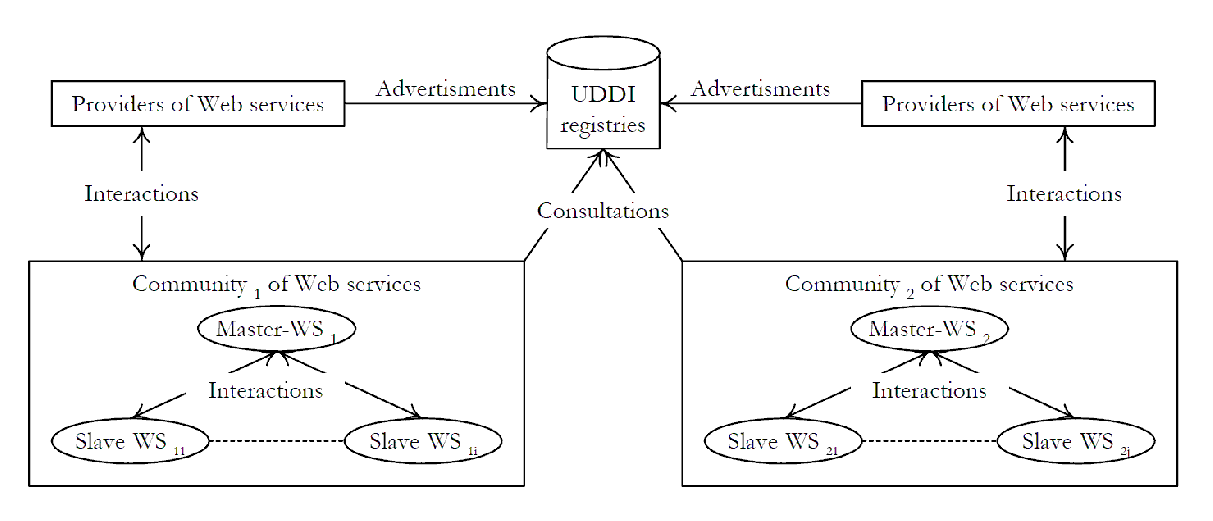
\includegraphics[width=16cm]{Figures/wsarch.eps}\label{wsarch}
            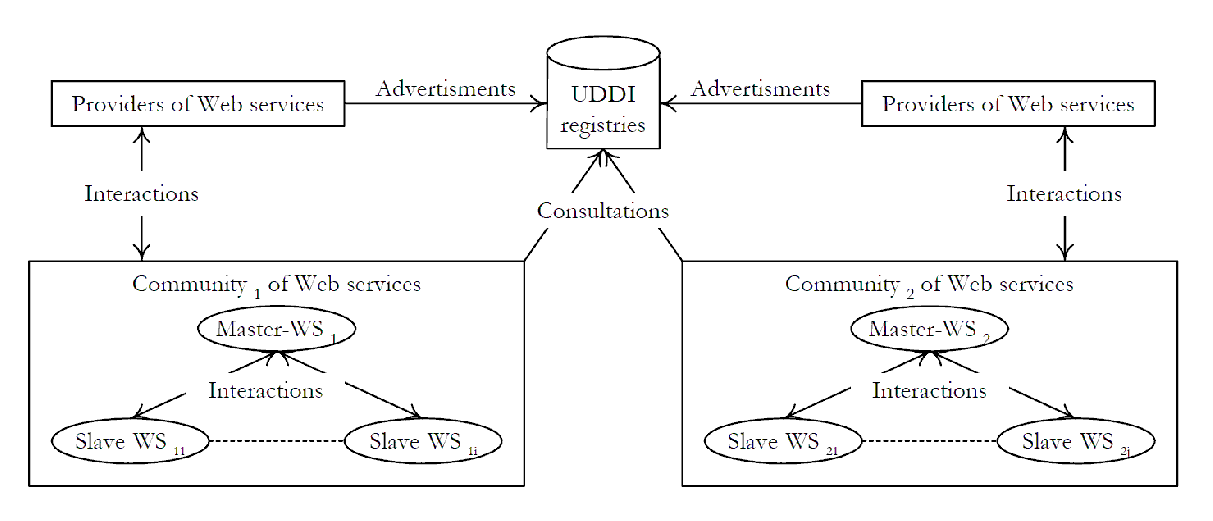
\includegraphics[width=16cm]{Figures/wsarch.eps}\label{wsarch}
            \caption{Communities of Web Services Architecture as Proposed in \cite{DBLP:journals/ijebr/MaamarSTBB09}}
            \end{center}
        \end{figure}

Figure 1 %\ref{wsarch}
depicts the basic architecture of
communities of web services. The main components of the
architecture are: 1) the providers of web services; 2) UDDI
registries; and 3) communities platform. Communities abstract the
same model of defining, announcing and invoking web services. They
also adopt the same protocols that standard web services use with
UDDI registries. UDDI is a platform-independent XML based registry
list which facilitates worldwide web service discovery.

%The master web service is responsible with communication with web
%service providers and discovery registries. It it responsible for
%task distribution, web service selection, community management,
%maintaining a healthy set of web services satisfying end users
%requests with high QoS. In communities, the masters web services
%can be dedicated web services playing the master role during the
%entire time of being in the community. This master web service is
%independently developed and never participates in any
%composition. The master web services can also be chosen out of
%normal web services already inside the community
%\cite{DBLP:journals/ijebr/MaamarSTBB09}.


\section{Cooperative Game Theory and Multi-Agent Systems}\label{sec:CGTMS}

%        Cooperative game theory provides a set of mathematical and optimization tools for multi-agent environments. These tools have been utilized in communication networks and service oriented computing literature, where nodes as rational agents try to reason strategically and maximise their benefit.

The theory of cooperative games is a branch of game theory that is a branch of game theory that studies
strategies of self-interested entities or agents in a setting
where those agents can increase their payoff by binding agreements
and cooperating in groups. We let $N$ be a set of players which
can form a group called a $coalition$. A \emph{coalitional game}
is a pair $G = (N, v)$, where $v$ is called a \emph{characteristic
function} $v: 2^N \to \mathbb{R}$, mapping the set of players of
the coalition to a real number $v(N)$, the worth of $N$. This
number usually represents the output or payoff or again the
performance of these players working together as coalition. If a
coalition $S$ is formed, then it can divide its worth, $v(N)$ in
any possible way among its members. The payoff vector $x \in
\mathbb{R}^N$ is the amount of payoff being distributed among the
members of the coalition $N$. The payoff vector satisfies two
conditions:

        \begin{itemize}
            \item $x_i \geq 0$ for all $i \in N$, and
            \item $\sum_{i \in N} x_i \leq v(N)$
        \end{itemize}

        The second criterion is called the \emph{feasibility} condition,
        according to which, the payoff for each agent cannot be more than
        the coalition total gain. A payoff vector is also \emph{efficient}
        if the payoff obtained by a coalition is distributed amongst the
        coalition members: $\sum_{i \in N} x_i = v(N)$. This definition of
        the characteristic function works in \emph{transferable utility}
        (TU) settings, where utility (i.e., payoff) is transferable from
        one player to another, or in other words, players have common
        currency and a unit of income that is worth the same for all players
        \cite{myerson1991game}.

        \noindent When dealing with cooperative games, two issues need to be
        addressed:
        \begin{enumerate}
            \item Which coalitions among all possible coalitions to form?
            \item How to reward each member when a task is completed?
        \end{enumerate}
        The following sections help address these two issues.

        \subsection{Cooperative Game Concepts}

            {\bf Definition 1 (Shapley value)} Given a cooperative game $(N,
            v)$, the \emph{Shapley value} of player $i$ is given by \cite{shapley_value}:
            \begin{equation}\label{eq:shapley}
            \phi_i(N,v) = \sum_{S \subseteq N \backslash \left\{i\right\} }
            \frac{|S|! (|N|-|S|-1)!}{|N|!} (v(S \cup \left\{i\right\}) - v(S))
            \end{equation}

            \emph{Shapley value} is a unique and fair solution concept for
            payoff distribution among the members of the coalition. It
            basically rewards members with the amount of marginal contribution
            they have to the coalition.  It checks the contribution of member $i$ by adding the agent, to all possible subsets
            of coalitions $S$, where $S \subseteq N\backslash\left\{i\right\}$. If he is added to the set $S$, his
            contribution to the coalition is $v(S \cup \left\{i\right\}) - v(S)$. Average marginal contribution of agent $i$'s
            is calculated by averaging this value over all possible subsets of $N$, in $Shapley value$ equation (\ref{eq:shapley}).

            %\subsubsection{Core}

            {\bf Definition 2 (Core)} A payoff vector $x$ is in the $core$ of
            a coalitional game $(N, v)$ if and only if:
            \begin{equation}\label{eq:core}
            \forall S \subseteq N, \sum_{x_i \in S} x_i \geq v(S)
            \end{equation}

            The core is basically a set of payoff vectors where no subset of
            players $S^\prime$ could gain more than their current payoff by
            deviating and making their own coalition $\sum_{i \in S^\prime}
            x_i \geq v(S^\prime)$. The sum of payoffs of the players in any
            sub-coalition $S$ is at least as large as the amount that these
            players could earn by forming a coalition by their own. In a
            sense, it is analogue to Nash equilibrium, except that core is
            about deviations from groups of entities. The core is the
            strongest and most popular solution concept in cooperative game
            theory. However, its computation is a combinatorial problem and
            becomes intractable as the number of players increases. The core
            of some real-world problem games may be empty, which means having
            the characteristic function of the game $(N,v)$, there might be no
            possible distribution of payoff assuring stability of subgroups.

            {\bf Definition 3 (Convex cooperative games)} A game $(N,v)$ with
            characteristic function $v(S)$ is convex if:
            \begin{equation}\label{eq:convex}
            v(S) + v(T) \leq v(S \cup T) + v (S \cap T), \forall S,T \subseteq
            N.
            \end{equation}

            According to a classic result by Shapley \cite{S1971cores}, convex
            games always have a non-empty core. We will use a variation of
            convexity condition in our algorithm to check whether our
            coalitions are stable.

            \subsubsection*{$\epsilon$-core}\label{s:epsilon}
            %\emph{$\epsilon$-Core:}
            %\\
            When the \emph{core} set of a game is empty, it means no coalition
            of players can gain anything by deviating. An outcome would be
            unstable if a coalition can benefit even by a small amount from
            deviating, which is a strong requirement. In fact, in some
            situations, deviations can be costly, or players may have loyalty
            to their coalitions, or even it can be computationally intractable
            to find those small benefits. It would only make sense for a
            coalition to deviate if the gain from a deviation exceeds the cost
            of performing the deviation. \emph{$\epsilon$-core} relaxes the
            notion of the core, and only requires that no coalition would
            benefit significantly, or within a constant amount($\epsilon$) by
            deviating (see Equation \ref{eq:core2}).

            \begin{equation}\label{eq:core2}
            \forall S \subseteq N, \sum_{x_i \in S} x_i \geq v(S) - \epsilon
            \end{equation}

            \subsubsection*{Coalition Structure Formation}\label{sec:coalition}

            Coalition structure formation is the problem of finding the best
            partition of web services into teams. In these settings, the
            performance of an individual service is less important than the
            \emph{social welfare} of the whole system, which is the sum of the
            values of all teams. Having the game $(N,v)$, a coalition
            structure $(CS)$ is \emph{socially optimal} if $CS$ belongs to set
            $\operatorname*{arg\,max}_{CS} v(CS)$ where $v(CS)$ is the sum of
            the values of all coalitions inside $CS$. $v(CS) = \sum_{C \in
            CS}v(C)$.
            %The outcome of a characteristic function game in coalition structure settings, consists of two parts; first a disjoint partition of players (agents) into coalitions, called a \emph{coalition structure} (CS) and second a \emph{payoff vector} as mentioned in cooperative game solution concepts, which distributes the value of each coalition among its members.


        %\subsection{Examples on Cooperative Game Solution Concepts}\label{sec:CWSDefinition}

\begin{example}\label{ex:simplecore1}
Consider a game $G = (N, v)$, with two players where $N = {1,2}$.
Each of these players can produce 5 units of output working alone
and by collaborating they can produce 20 units worth of output.
Therefore we have: $v({1}) = 5, v({2}) = 5, v({1,2}) = 20$. The
$core$ of the game, which is the set of all possible distribution
of gain among players guaranteeing stability is: $core(N,v) =
\{(x_1,x_2) \in R^2 | x_1 >= 5, x_2 >= 5, x_1 + x_2 = 20\}$, as
illustrated in Figure 2. Distributing the 20 units of income,
among these two players, for all the points in the line will make
outcome stable, since non of these players can gain more than 5 by
working alone. However although they have same qualities, the core
can suggest a stable outcode where one agent can earn three times
more than the other agent: $\{5,15\}$. As mentioned in previous
section, $core$ result may not be fair, the $core$ only considers
stability. However, \emph{Shapley value} considers fairness.
According to equation \ref{eq:shapley}, the two  workers should
each share 10 units of income, since they have the same marginal
contribution to all subsets of the coalition. As you can see the
distribution vector of $\{10,10\}$ is also a member in $core$ set.
Later we are going to show if $core$ of a coalition game is not
empty, and game is convex, the shapely value lies within $core$
set.
\end{example}

            \begin{figure}
                \begin{center}
                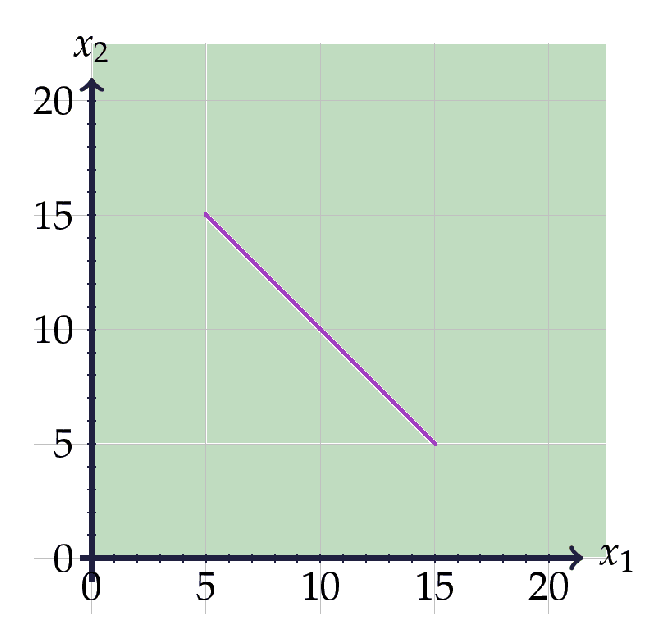
\includegraphics[width=3in]{Figures/excore.eps}\label{fig:coreex1}
                \caption{Core of the 2-player game of example \ref{ex:simplecore1}}
                \end{center}
            \end{figure}


            \begin{example}\label{ex:simplecorealpha}
                In this example, we want to analyse games under conditions which core can be empty. Consider a game $G = (N, v)$,  where $N = {1,2,3}$ and $v(\{i\}) = 0$, $v(\{Ci\}) = \alpha for |C| = 2$ and $v(\{N\}) = 1$. The $(x_1,x_2,x_3)$ distribution vector according to equation \ref{eq:core}, is in $core$ if $x_i \geq 0$ which implies each player will get more than 0 which they would when working alone and $\forall i, \forall j, x_i + x_j \geq \alpha $ which implied any pair of players will get more than $\alpha$ which they would earn if they worked in pair without the third player and finally $\sum_{i \in N} x_i = 1$ which implied all the gain is distributed among the three players. Based on these three equations we have, $\forall i \in N 0 \leqslant 1 - \alpha$ and $\sum_{i \in N} x_i = 1$. By summing first equation for all three platers, we conclude $Core (N,v)$ is nonempty iff $\alpha \leqslant \frac{2}{3}$. When alpha is more than $\frac{2}{3}$, the contribution of third player is not good enough to justify the group of three players working together. The third player will increase the revenue with less then $\frac{1}{3}$, and the other two players, both can get better share of revenue if they work together. This is why the group of three players working together when $\alpha > \frac{2}{3}$ is not stable.
            \end{example}

            %\begin{example}\label{ex:simplecore2}
%
%                An example which has closely resembles our community service model is the \emph{Single landowner and landless workers} example.
%                This example was introduced in \cite{GVK369342747} and represents the \emph{landowner} entity which is providing jobs and \emph{landless workers} who cannot do anything by themselves and need to work with a landowner to gain revenue (payoff).
%
%                In this game, land is owned by a single person, the \emph{landowner}. We refer to the other people as \emph{workers}. In this case we have a game there the set of players are the landowner and the $m$ workers, possible actions for coalitions with only workers would be distributing the zero output for all where no member receives any output. The set of actions of a coalition $S$ consisting of the landowner and $k$ workers would be the set of all $S$-allocations of the output $f(k+1)$ among the members of $S$. The preference of each player would be the amount of out she obtains.
%
%                In this game the action $a_{N}$ of the grand coalition in which the landowner obtains all the output $f$(n)
%                is in the core: all coalitions that can produce any output include the landowner, and none of these
%                coalitions has any actions that makes her better off than she is in $a_{N}$.
%
%                For any value of n The core contains actions in which the workers receive some output.
%                The workers need the landowner to produce any output, but the landowner
%                also needs the workers to produce more than $f$(1), so stable actions of the grand coalition exist in which the
%                workers receive some output. Take the landowner to be player 1, and consider the action $a_{N}$ of the grand
%                coalition in which each player $i$ obtains the output $x_{i}$, where $x_{1}+...+x_{n}=f(n)$. Under what conditions
%                on  $(x_{1},..,x_{n})$ is $a_{N}$ in the core? Because of my assumption about the shape of the function $f$, the
%                coalitions most capable of profitably deviating from $a_{N}$ consist of the landowner and every worker but one.
%                Such a coalition can, by itself, produce $f(n-1)$, and it may distribute this output in any way among its members.
%                Thus for a deviation by such a coalition not to be profitable, the sum of $x_{i}$ and any collection of $(n-2)$ other
%                $x'_{i}$s must be at least $f(n-1)$. That is, $(x_{1}+...+x_{n})-x_{i}\geq f(n-1)$ for every $j=2,..,n$. Because
%                $x_{1}+...+x_{n}=f(n)$, we conclude that $x_{i}\leq f(n)-f(n-1)$ for every player $j$ with $J\geq 2$ (i.e. every worker).
%                That is, if $a_{N}$ is in the core then $0\leq x_{j}\leq f(n)-f(n-1)$ for every player $J\geq 2$. In fact, every such action
%                is in the core, as you are asked to verify in the following exercise.
%
%            \end{example}

%          Core of landowner-worker game: Check that no coalition can improve upon any action of the grand
%          coalition in which the output received by every worker is nonnegative and at most $f(n)-f(n-1)$. (Use the fact that
%          the form of $f$ implies that $f(n)-f(k)\geq (n-k)(f(n)-f(n-1))$ for every $k\leq n$.)

%          We conclude that the core of the game is the set of all actions of the grand coalition in which the output $x_{i}$
%          obtained by each worker $i$ satisfies $0\leq x-{1}\leq f(n)-f(n-1)$ and the output obtained by the landowner is the
%          difference between $f(n)$ and the sum of the worker's shares. In economics jargon, $f(n)-f(n-1)$ is a worker's
%          ``marginal product". Thus in any action in the core, each worker obtains at most her marginal product.

%          The worker's shares of output are driven down to at most $f(n)-f(n-1)$ by competition between coalitions consisting
%          of the landowner and workers, in cahoots with the landowner, can deviate and increase their share of output. That is,
%          each worker's share of output is limited by her comrade's attempts to obtain more output.

%          The fact that each worker's share of output is held down by interworker competition suggests that the workers might
%          be better off if they were to agree not to join deviating coalitions \emph{except as a group}.

        %\subsection{Cooperative Games in Service Oriented Computing}\label{sec:CWSArchitecture}

        \subsection{Stability of Coalitions}

        Core stability is a highly desirable property however in many problems it is not achievable. It would be more ideal to maintain a set of somewhat stable payoffs when the core is empty. There are several approaches to achieve this goal. One may drop the stability requirement and focus on other types of solutions for which a payoff division is guaranteed to exist. Two well known solution concepts in this category are \emph{nucleolus} \cite{schmeidler_nucleolus_1969} and the \emph{bargaining set} \cite{Davis67existenceof}. They try to minimize some measure of unhappiness in the game for the agents.

        Another approach to stabilize the game can be achieved via external subsides. When \emph{Core} is empty it means the game is not stable since the coalition is unable to generate enough revenue to satisfy the demands of each subset of agents. An external party that is interested in stabilizing the game provides a subsidy to the agents if they form the grand coalition, and thus a value of $\lambda v(C)$ is divided among them, where $\lambda \geq 1$. Clearly any game can be stabilized using a large enough $\lambda$, however the external party would be interested in the minimal subsidy required in order to stabilize the game.

        A community can also be stabilized by relaxing the core constraints. According to \emph{Core}, an outcome is unstable if a coalition can benefit even by a small amount from deviating, which is a strong requirement. In fact, in some situations, deviations can be costly, or players may have loyalty to their coalitions, or even it can be computationally intractable to find those small benefits. It would only make sense for a coalition to deviate if the gain from a deviation exceeds the cost of performing the deviation. \emph{$\epsilon$-core} relaxes the notion of the core, and only requires that no coalition would benefit significantly, or within a constant amount($\epsilon$) by deviating (see Equation \ref{eq:core3}).

           \begin{equation}\label{eq:core3}
               \forall S \subseteq N, \sum_{x_i \in S} x_i \geq v(S) - \epsilon
           \end{equation}

        Alternatively, $\epsilon$ can be thought of as a \emph{tax} imposed on a coalition should it choose to deviate. This can again be seen as an external party, trying to stabilize the coalition by imposing some \emph{tax} on deviation. Taxation and subsiding as methods of stabilizing cooperative games have been studied in \cite{RePEc:spr:jogath:v:38:y:2009:i:1:p:3-16, Bachrach:2009:CSC:1692490.1692502, conf/ijcai/MeirRM11}.


        \subsection{Representation and Complexity Issues}\label{sec:CWSArchitecture}

        Shapely value is the unique ``fair'' way to distribute the total surplus generated by the coalition, among all the players.
        The nature of the Shapley value is combinatorial, as all possible orderings to form a
        coalition needs to be considered. This computational complexity can sometimes be
        an advantage as agents cannot benefit from manipulation. For example, it is NP-complete
        to determine whether for a bunch of agents to collude and make their own coalition and guarantee
        an increase in payoff of all participants \cite{conf/aaai/YokooCSOI05}.
        There are some representations that allow us to compute the Shapley value efficiently by reducing the input size of the problem.
        One example is \emph{Induced subgraph games}
        which was introduced by Deng and Papadimitriou \cite{Deng94}. In this representation, players are represented by graph nodes, and
        their valuation function should be the sum of weights of all edges between the node and all its neighbors. It is a succinct representation, using
        an adjacency matrix, which needs only $O(n^2)$ space to store all the input, which is a major improvement from $O(2^n)$ because
        if weights of all the edges in graph are all positive, the Shapley value can be computed in time $O(n^2)$.
        However, this representation is not complete, some games cannot be represented by a induced subgraph game \cite{conf/aaai/YokooCSOI05}.

        Ketchpel introduces the Bilateral Shapley Value (BSV) \cite{conf/aaai/Ketchpel94a} for coalition games with general valaution functions.
        It reduces the combinatorial complexity of the computation of the Shapley value, breaking the community to multiple disjoint set.
        With backtracking and dynamic programming like methods, they merge and store the marginal contribution of disjoint coalitions,
        reducing the overall complexity of the algorithm. However, the solution is still NP-Complete and BSV time and space complexity grows exponentially.

        In order to make cooperative game concepts practical in real world application, we have proposed an approximation multi-layer
        algorithm useful for service orinted computing settings. Our excrements illustrate, these algorithms can provide
        applicable and near optimal solutions for real world applications.


\section{Related Work}\label{sec:BRRelatedWork}

\subsection{Communities of Web Services}\label{sec:communities_rel}

Here we introduce the related research work regarding the engineering and formation
of communities of web services. In \cite{DBLP:journals/internet/BenatallahSD03}, Benatallah et al.
defined communities as \emph{Service Containers} that aggregate
substitutable web services providing a common functionality (same
set of operations). They abstracted \emph{Service Containers} as
web services that are created, advertised, discovered and invoked
just as elementary web services. The \emph{Container} is
considered as a manager that is responsible for web service
selection upon receiving a request on run-time. The authors have
proposed a scoring service based on non-functional requirements of
the request and web service capabilities to dynamically chose the
web service to perform the requested task. A similar concept was
proposed by Maamar et al. in
\cite{DBLP:journals/ijebr/MaamarSTBB09}. The authors introduced
web services communities as a collection of web services with a
common functionality but different QoS properties. A community
manager, upon receiving a request, delegates the request to one of
its current members. The choice is based on the performance
history and quality metrics of each web service. The authors have
proposed an efficient global web service selection algorithm in
order to approach quality constraints and preferences for
composite services which require aggregation of different types of
services to satisfy the user.

Benslimane et al. \cite{Liris-2770} have proposed a multi-layer
approach grouping similar Web services into communities and having
an interface implemented as an abstract web service for accessing
the community on top of the community layer. The interactions
between composite, management and community layers and the
bindings are performed by a generic driver called Open Software
Connectivity (OSC).

In \cite{managing-hela-jalel}, Limam and Akaichi have proposed web
service communities with centralized access across distributed web
services. They have proposed a framework for web service
management, query resolution among communities and a query caching
mechanism executed by the manager to improve the performance of
query resolution process among many distributed communities. The
key idea is to cache previous computed results for answering
future queries.


Maamar et al. initially in \cite{conf/webist/MaamarLBTS07} and
then comprehensively in \cite{DBLP:journals/ijebr/MaamarSTBB09}
proposed an architecture utilizing \emph{Contract-Net} protocol
for engineering task distribution within communities of web
services. The protocol is centrally executed by the community
manager. This architecture has been further developed in
\cite{CSTintercommunity, conf/IEEEscc/BenharrefSBB11,
conf/IEEEscc/KhosravifarBMMT10, conf/aina/LimTM11}. Two types of
roles have been distinguished for community members: masters and
slaves. Master web services and community managers that lead
communities and are responsible for membership management. They
can invite and convince slave web services to join the community,
and attract new slave web services to their communities by
awarding them better payoff. Moreover, they can eject some slave
members from the community to improve its overall reputation if
these members are misbehaving or cannot provide the promised QoS.

In \cite{Medjahed05adynamic}, Medjahed and Bouguettaya have
developed a community as a ``cluster'' that groups Web services
based on a specific area of interest. All web services in a given
community share the same functionality. These communities are
created by \emph{third party community providers} which use the
\emph{community ontology} as a template and define a set of
operations that all web services within a community should
provide. Using semantic analysis on web service operations, web
services either find and join a community with similar
functionality or create a new operation description for a new
community. The authors have described the concept of
\emph{community agents} associated to \emph{community providers}.
A community agent is responsible, among other things, of the
registration of services with the community. An example of a
community that provides health care services to senior citizens
has been used. In this example, a governmental entity is needed to
check the health care standards used by the members before
authorizing them to be part of the community. Such a central
entity is represented by the community agent. Thus, community
agents are playing the role of community managers. In a close work
\cite{Zeng:2003:QDW:775152.775211}, Zeng et al. have described a
global planning selection algorithm and a delegation algorithm to
be run when a request to execute an operation is received by the
community. This needs a central entity to run those algorithms.
Such entity plays the same role as the community coordinator or
manager. 

\subsection{Web Services Community Formation}\label{sec:communities_for_rel}

Most of the recent work on communities of services are either
user-centric and focus on user satisfaction
\cite{Chun02user-centricperformance} or system-centric and focus
on the whole system throughput, performance and utilization. There
are many contributions in distributed, grid, cluster and cloud
services which are system-centric. However, in real world
environments and applications, both users and service providers
are self-interested agents, aiming to maximize their own profit.
In those environments, both parties (users and services) will
collaborate as long as they are getting more benefits and payoff.

In this direction, recently \cite{DBLP:conf/IEEEscc/LimTMB12,
DBLP:conf/IEEEscc/KhosravifarABT11, 10.1109/TSC.2012.12} proposed
mechanisms to help users and services maximize their gain. A
two-player non-cooperative game between web services and community
master was introduced in
\cite{DBLP:conf/IEEEscc/KhosravifarABT11}. In this game-theoretic
model, the strategies available to a web service when facing a new
community are requesting to join the community, accepting the
master's invitation to join the community, or refusing the
invitation to join. The set of strategies for communities are
inviting the web service or refusing the web service's join
request. Based on their capacity, market share and reputation, the
two players have different sets of utilities over the strategy
profiles of the game. The main limits of this game model are: 1)
its consideration of only three quality parameters, while the
other factors are simply ignored; and 2) the non-consideration of
the web services already residing within the community. The game
is only between the community master and the new web service, and
the inputs from all the other members and their influence on the
master's decision are simply ignored. The consideration of those
inputs and this influence factor is a significant issue as
existing web services can lose utility or payoff because of the
new member, which can result in an unhealthy and unstable group.
The problem comes from the fact that the existing members should
collaborate with the new web services, so probably their
performance as a group can suffer. Existing members may even
deviate and try to join other communities if they are unsatisfied.
Those considerations of forming stable and efficient coalitions
are the main contributions of our research work.

In \cite{DBLP:conf/IEEEscc/LimTMB12}, a 3-way satisfaction approach
for selecting web services has been proposed. In this approach,
the authors proposed a web service selection process that the
community masters can use. The approach considers the efficiency
of all the three involved parties, namely users, web services and
communities. In this work, it is shown how the gains of these
parties are coupled together using a linear optimization process.
However, the optimization problem in this solution tends to
optimize some parameters considering all web services regardless
of their efficiency and contribution to the community's welfare.
Moreover, there are no clear thresholds for accepting or rejecting
new web services. The solution of the optimization problem could,
for instance, suggest web services already residing within the
community to increase or decrease their capacity to cover up the
weakness of other parties in the system. However, a high
performing web service could deviate anytime it finds itself
unsatisfied within the community instead of adjusting its service
parameters.

In \cite{10.1109/TSC.2012.12}, a cooperative scheme among
autonomous web services based on coalitional game theory has been
introduced. The authors have proposed an interesting algorithm to
reach individually stable coalition partition for web services in
order to maximize their efficiency. The communities choose new web
services on the promise that it would benefit the community
without decreasing any other web service's income. In the proposed
model, the worth of community is evaluated with high emphasis on
the availability metric and considering price and cost values
only. The community structure is based on a coordination chain,
where a web service is considered as a \emph{primary} web service
and the community task-distribution method initially invokes the
primary web service and only if the primary web service is
unavailable, the method invokes the next backup web services as
they are ordered in the coordination chain. We believe that this
coordination chain limits the cooperation power as it introduces a
sort of hierarchy. However, in pure and open cooperative models,
such as the one we propose in this thesis, active cooperation
activities engaging simultaneously many agents so that they can
perform the tasks more efficiently are being used. Moreover, if
the availability is high, which is the case nowadays with the
recent advancements in cloud and hardware infrastructures, the
backup web services will end-up having a very low chance of
getting jobs, especially the ones further in the chain. This will
results in a considerable waste of web services capabilities.

\subsection{Coopetitive Behaviour Within Communities of Web Services}\label{sec:coopetetive}

At the best of our knowledge, there is no work in the literature of service and agent computing addressing the issue of coopetition strategies and when to cooperate or to compete. However, some relevant proposals to our proposed model are the ones that address service selection and task allocation mechanisms. In many frameworks proposed in the literature, service selection and task allocation are regulated based on the reputation parameter \cite{Bentahar:2012:ARA:2343124.2343267,DBLP:journals/jwsr/RosarioBJ10,Ruth_Tu_2007-7,journals/kbs/Yahyaoui12}. In \cite{HuangCommunications}, the authors propose a framework to match potential benefits of services while cooperating with one another. The interesting idea is to consider the benefits under four categories: innovation and learning, internal business process, customer, and financial benefits. Innovation and learning perspective focuses on the knowledge, skills, and systems needed to improve the business continually. Necessary factors to build strategic capabilities and efficiency in addressed in internal business process. Values that customers seek are considered in \emph{customer perspective} and financial performance to maximize the shareholder value are analyzed in \emph{financial perspective}. Their goal is to design the framework for cooperating web services, inline with business strategy of firms in IT industry. In \cite{alchieri:a}, the authors present a dependable framework for cooperative service agents that is based on the tuple space coordination model. The intrusion-tolerant perspective is emphasized in the paper where several security mechanisms are developed to enable a reliable coordination system. %In \cite{Maximilien2}, authors propose %ontology for quality of service. Users compute the web services' %reputation using ratings.
The proposed frameworks mostly aim to facilitate the coordination mechanism between services. However, the opposite strategy of competing is not analyzed where services might be more successful when competing within the same group. In fact, services are not always willing to cooperate even if they have some common goals, particularly when they operate within groups such as communities. In such a context, service agents can follow different interacting strategies and have to decide when to compete and when to cooperate so that their ultimate goal, maximizing their incomes, can be better achieved. In our framework, we analyze those different strategies to help services in their decision making process when these
agents function within communities.
%We summarize most of %these proposals and concentrate on strategic decision making %system that ranks web services in the community and analyze their %effective interacting strategies to accomplish continuous %requested tasks.
We enable service agents to reasonably evaluate and decide over their coopetition strategies, which means deciding when to compete and when to cooperate.



Furthermore, there are a number of related proposals that take
into account the correlation between (web) services and the ways
these services coordinate their actions to accomplish the required
tasks. In \cite{Jurca2007b,Jurca2005d,DBLP:conf/wise/MalikB07,Maximilien:2001:REW:844331.844335,journals/kbs/Yahyaoui12}, the
authors propose to rank services based on their reputation in the
system and to use this ranking as a means to facilitate
cooperation of services. In those models, services rely on one
another on the basis of the reputation ranking system, using,
among other parameters, the QoS \cite{Tao:2012:NPA:2064113.2064479}. There are
other models that facilitate cooperation mechanisms among services
using various techniques. Examples of those techniques include 1)
coordination between two types of behaviors associated with
component services: operational and control behaviors
\cite{DBLP:journals/ijwgs/YahyaouiMB10}; 2) Services-based workflows \cite{Wu2011}; 3)
transaction-based approaches \cite{Gao:2011:STI:2093449.2093450,DBLP:conf/icws/RosarioBHJ07}; 4) agent
coordination mechanisms \cite{DBLP:journals/aamas/CharifS13,DBLP:journals/apin/Gutierrez-GarciaS13}; 5)
logical techniques \cite{Okutan:2010:MAA:1805335.1805430,tang:automatic}; and 6) community models,
which are virtual structures that aim at increasing the visibility
of services and facilitating their discovery and composition by
hosting and gathering services having similar or complementary
functionalities but different QoS parameters
\cite{DBLP:journals/jwsr/KhosravifarBMT10}. %There are also some frameworks
%\cite{Ferguson,Ferguson2} that consider game-theoretic analysis on
%the expected payoffs obtained via different acting strategies.
However, deciding about which strategy to choose when services are
competing but still need to cooperate to accomplish complex tasks
has not been addressed and kept as open issue in all these
proposals as faithfully argued in
\cite{1fd085d030db49d9ad024f89d13faff3,DBLP:conf/icsoc/KhosravifarAABMO12}.

%All the proposed frameworks share a common aspect, which is providing the solution based on assumption of having complete information of all services and performing evaluations based on a large number of input each time they want to adopt a strategic decision making process.
%So basically These solutions generally suffer from high complexity, which makes decision making impossible in an on-demand fashion, or they simplify important aspects to make it practical in the real world, thereby hurting the decision making performance. We address this issue by introducing DDM a framework that operates based on a trained model that regulates web service agents' decision making process in terms of cooperating with one another. After being trained, web services get to compute expectations as utilities they would gain while cooperating with communities of different characteristics. Therefore web services and communities can make prudent decisions when inviting a web service to join or accepting a join inquiry initiated from a web service. In general, DDM equips web services with efficient methods for foreseeing how their choices will impact their long-term and short-term goals; therefore, opting for best decision available.


\section{Conclusive Remarks}

In this thesis, as the first contribution, we will tackle the issue of community formation in an efficient way for all the web services and communities involved. We will use game theory to propose a cooperative game model for the aggregation of web services within communities. The solution concepts of our cooperative game seeks to find efficient ways of forming coalitions (teams) of web services so that they can maximize their gain and payoff, and distribute the gain in a fair way among all the web services. Achieving fairness when the gain is distributed among the community members is the main factor to keep the coalition stable as no web service will expect to gain better by deviating from the community. In other words, the coalition is made efficient if all the members are satisfied. We first propose a representation function for communities of web services based on their QoS attributes. By using this function, we can evaluate the $worth$ of each community of web services. When facing new membership requests, a typical community master checks whether the new coalition having the old and new set of web services will keep the community stable or not. The community master will reject the membership requests if it finds out that the new coalition would be unstable, preventing $any$ subset of web services from gaining significantly more by deviating from the community and joining other communities or forming new ones. The computation of solutions for cooperative game theory problems is combinatorial in nature and proven to be NP-complete \cite{Algorithmic}, making this computation impractical in real world applications. However, using the concepts of coalition stability, we propose approximation algorithms running in polynomial time providing web services and community masters with applicable and near-optimal decision making mechanisms.

Next we will tackle the issue of distributed model of web services and propose a decision model for scenarios where information is incomplete. We proposed a training model for the problem of membership management of communities of web services. Using the traning model we created a decision making profile for each community and web service involved which provides them with a set of feasible and utility increasing moves. This utilized our web services with efficient methods of foreseeing how their choices of actions would impact their long-term and short-term goals, therefore they opted for best decision available. The ultimate goal is to choose the best decision when it comes to communities formation, among many possible short-term rational and utility increasing choices. The experimental results show that our algorithms provide web services and community owners, in real-world-like environments, with applicable and near-perfect decision making mechanisms. The results of experiments using real data samples support the need for a long-term training model in a successful decision making process.

In our last contribution, the focus is on internal community management. We proposed a game-theoretic based model to analyze the best efficiency characteristics for the active services in open networks. The proposed framework considers the chances of web services in joining a community in different cases with truthful and lying information service agents. The proposed game analyzes the existing Nash equilibrium and situations where the maximum payoff is obtained.
